%----------------------------------------------------------------------
% 文獻討討
%----------------------------------------------------------------------
\chapter{研究理論}

\section{FDTD}
在計算電磁學的研究中，由 Kane S. Yee 於 1966 年提出的時域有限差分法（Finite-Difference Time-Domain, FDTD)。該方法的基本核心，FDTD是在不考慮自由電荷與自由電流的各向同性介質環境下，在時域（Time domain）中直接求解主導電磁波傳播的麥克斯韋時域旋度方程（Maxwell's time-dependent curl equations）偏微分方程組可寫作：
\renewcommand{\theequation}{\arabic{chapter}.\arabic{equation}}是
\begin{align}
	\nabla \times \mathbf{E} &= -\mu \frac{\partial \mathbf{H}}{\partial t} \\[1em]
	\nabla \times \mathbf{H} &= \varepsilon \frac{\partial \mathbf{E}}{\partial t}
\end{align}
其中，$\mathbf{E}$ 表示電場強度，$\mathbf{H}$ 表示磁場強度，$\varepsilon$ 與 $\mu$ 則分別對應該介質環境的介電常數與磁導率。在於將上述連續的空間與時間進行網格化離散（Discretization），藉此精確捕捉電磁波與非均勻奈米結構交互作用時的瞬態動態演變。\\
為了將這些連續的偏微分方程轉化為計算機可執行的代數遞迴式，該方法引入了經典的「伊氏晶格（Yee cell）」交錯幾何架構。在網格空間中，電場分量與磁場分量交錯坐落於不同的位置，這種幾何配置使得空間中的電場與磁場分量相互環繞，在空間結構上直接對應了麥克斯韋方程組中的旋度關係。此外，電場與磁場在時間軸的更新上也錯開了半個時間步長（$\Delta t / 2$），形成交替推進的「蛙跳式（Leap-frog）」時間演進機制。在此架構下，下一時刻的場量強度完全由當前已知場與鄰近網格的空間差分共同決定，實現了電磁波在空間中隨時間推移的動態傳播模擬。
\begin{figure}[H]
	\centering
	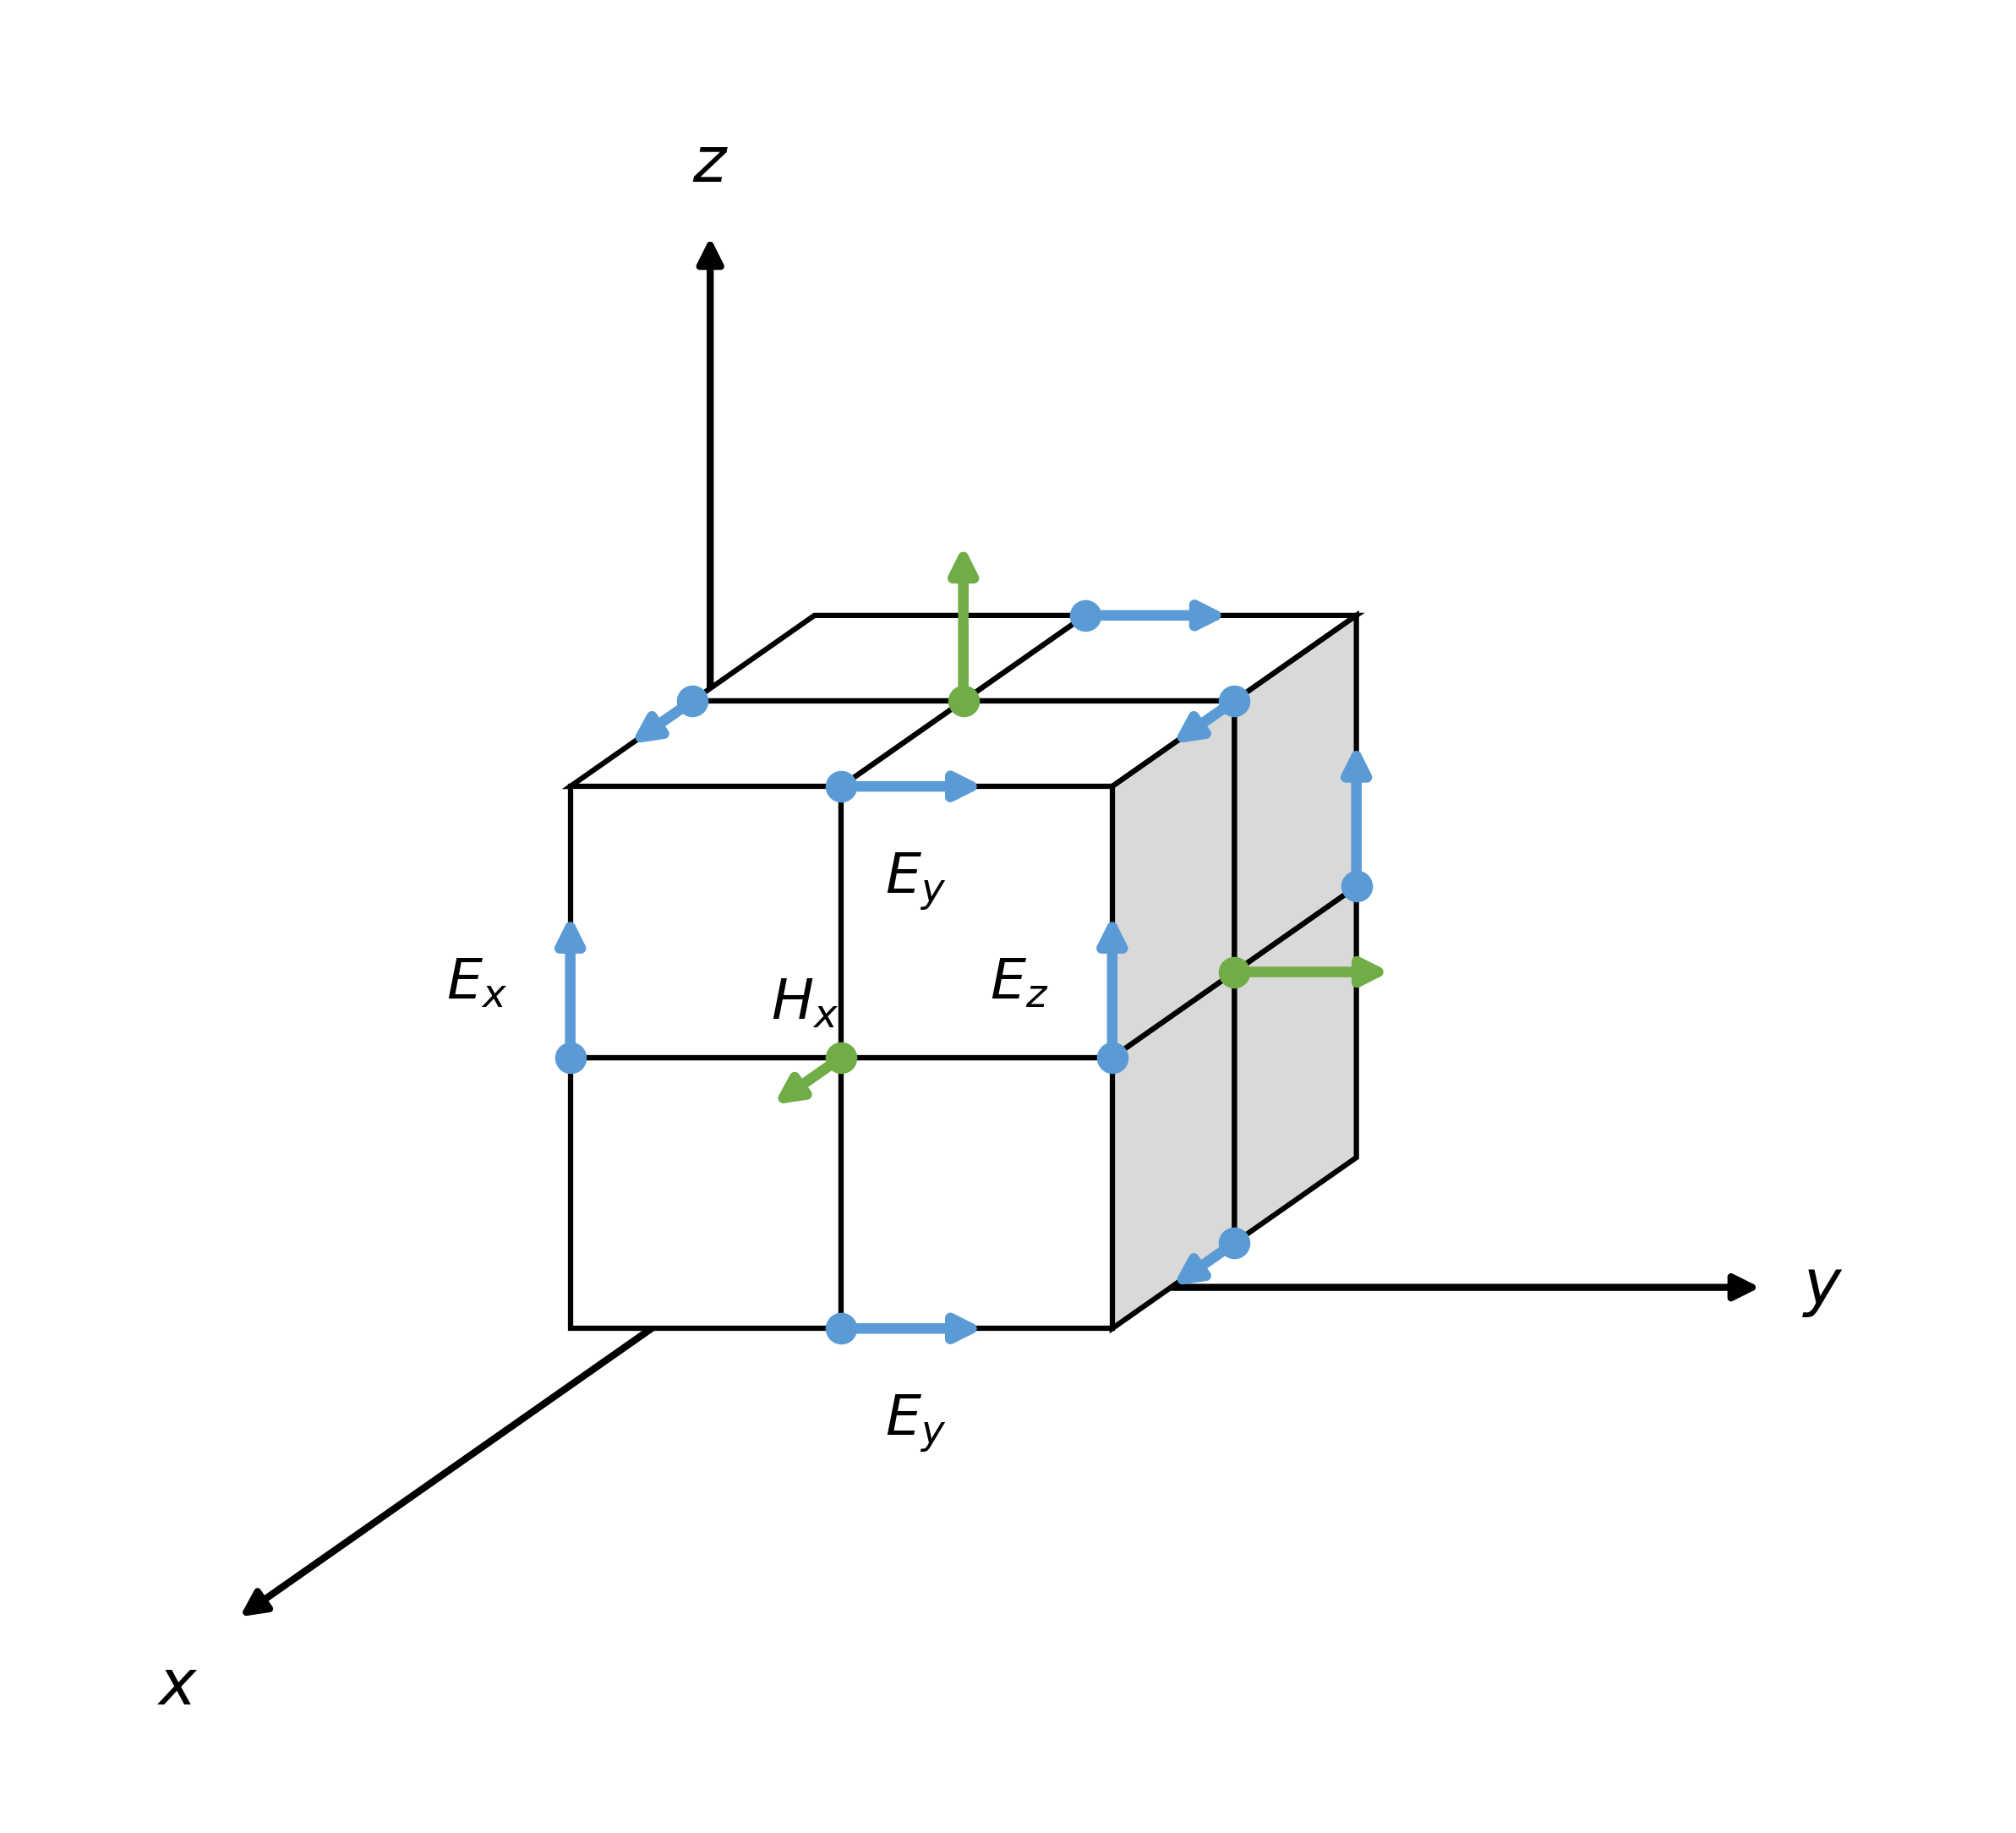
\includegraphics[width=0.6\textwidth]{Figures/YeeGrid.png}
	\caption{Yee lattice unit cell}
	\label{fig:yee_cell}
\end{figure}
然而，由於計算機的記憶體與運算資源有限，我們無法在無限大的空間中進行模擬，必須建立一個有限大小的計算區域（Computational domain）。當電磁波傳播到這個人為截斷的模擬邊界時，會因為介質不連續而產生強烈的非物理性反射，這些二次反射波會回頭干擾原本模擬區域內的場型，導致結果失真。為了徹底解決這個邊界反射問題，模擬中必須配置完美匹配層（Perfectly Matched Layer, PML）作為吸收邊界條件。\\
在技術特點上，FDTD 最大的優勢在於其天然的寬頻分析能力。模擬時只需要輸入單個時域的高斯脈衝，最後再透過傅立葉轉換，就能用一次模擬直接解析出很寬波長範圍內的光譜（像是穿透、反射和吸收光譜），不需要像頻域方法那樣對每個波長逐點計算。現在配合 GPU 加速，運算速度大幅提升，因此它被廣泛用來設計奈米光子學元件、表面電漿子結構、光子晶體和超穎材料。另外，它也很適合與伴隨場方法結合，用來做光學元件的拓撲優化與反向設計。

% ─────────────────────────────────────────
\section{激子多體理論與 Bethe-Salpeter 方程式（BSE）}
\label{sec:theory_BSE}
% ─────────────────────────────────────────
在單層過渡金屬二硫族化合物（TMD-MLs）中，由於二維量子侷限系統的面外介電屏蔽效應微弱，顯著增強的庫侖交互作用使電子與電洞間的束縛能非常強 \cite{Chernikov2014}。傳統基於密度泛函理論（DFT）的單粒子能帶架構僅能描述獨立載子的準粒子（Quasiparticle）能量，無法有效捕捉電子與電洞之間的庫侖相干束縛態。因此，若要定量描述二維系統中的激子多體效應（Many-body effects），必須從多體微擾理論出發，首先構建激子系統的多體漢米爾頓量算符 $\hat{H}^{X}$ \cite{Lin2024Phd,Haug2009}：
在單層過渡金屬二硫族化合物（TMD-MLs）中，由於二維量子侷限系統的面外介電屏蔽效應微弱，顯著增強的庫侖交互作用使電子與電洞間的束縛能非常強 \cite{Chernikov2014}。傳統基於密度泛函理論（DFT）的單粒子能帶架構僅能描述獨立載子的準粒子（Quasiparticle）能量，無法有效捕捉電子與電洞之間的庫侖相干束縛態。因此，若要定量描述二維系統中的激子多體效應（Many-body effects），必須從多體微擾理論出發，構建激子系統的多體漢米爾頓量算符 $\hat{H}^{X}$ \cite{Lin2024Phd,Haug2009}：
\begin{equation}
	\hat{H}^{X} = \hat{H}_0 + \hat{H}_{\mathrm{eh}}^d + \hat{H}_{\mathrm{eh}}^x
	\label{eq:H_exciton_total}
\end{equation}
在二次量化表象下，各個多體算符項可分別嚴格表示為 \cite{Lin2024Phd,Haug2009}：
\begin{align}
	\hat{H}_0 &= \sum_{c\mathbf{k}}\epsilon_{c,\mathbf{k}}\hat{c}_{c,\mathbf{k}}^{\dagger}\hat{c}_{c,\mathbf{k}} - \sum_{v\mathbf{k}}\epsilon_{v,\mathbf{k}}\hat{h}_{v,-\mathbf{k}}^{\dagger}\hat{h}_{v,-\mathbf{k}} \label{eq:H0_op} \\
	\hat{H}_{\mathrm{eh}}^d &= -\sum_{\mathbf{k}_{\mathrm{ex}}}\sum_{vck}\sum_{v'c'k'} V_{\mathbf{k}_{\mathrm{ex}}}^d(vc\mathbf{k}, v'c'\mathbf{k}') \, \hat{c}_{c,\mathbf{k}+\mathbf{k}_{\mathrm{ex}}}^{\dagger}\hat{h}_{v,-\mathbf{k}}^{\dagger}\hat{h}_{v',-\mathbf{k}'}\hat{c}_{c',\mathbf{k}'+\mathbf{k}_{\mathrm{ex}}} \label{eq:Hd_op} \\
	\hat{H}_{\mathrm{eh}}^x &= \sum_{\mathbf{k}_{\mathrm{ex}}}\sum_{vck}\sum_{v'c'k'} V_{\mathbf{k}_{\mathrm{ex}}}^x(vc\mathbf{k}, v'c'\mathbf{k}') \, \hat{c}_{c,\mathbf{k}+\mathbf{k}_{\mathrm{ex}}}^{\dagger}\hat{h}_{v,-\mathbf{k}}^{\dagger}\hat{h}_{v',-\mathbf{k}'}\hat{c}_{c',\mathbf{k}'+\mathbf{k}_{\mathrm{ex}}} \label{eq:Hx_op}
\end{align}
此處，$\hat{H}_0$ 為自由載子的準粒子動能項，$\hat{H}_{\mathrm{eh}}^d$ 為電子--電洞直接庫侖交互作用項，$\hat{H}_{\mathrm{eh}}^x$ 則為電子--電洞交換交互作用項 \cite{Haug2009}。$\hat{c}_{c,\mathbf{k}}^{\dagger}$（$\hat{c}_{c,\mathbf{k}}$）為導帶電子的創生（湮滅）算符，$\hat{h}_{v,-\mathbf{k}}^{\dagger}$（$\hat{h}_{v,-\mathbf{k}}$）為價帶電洞的創生（湮滅）算符，$\mathbf{k}$ 為載子的單粒子波向量，而 $\mathbf{k}_{\mathrm{ex}}$ 則代表激子的質心動量（Center-of-mass momentum）\cite{Lin2024Phd}。準粒子動能 $\epsilon_{c,\mathbf{k}}$ 與 $\epsilon_{v,\mathbf{k}}$ 由單粒子能帶結構決定 \cite{Lin2024Phd}。其交互作用核中直接項與交換項的散射矩陣元分別定義為 \cite{Lin2024Phd,Haug2009}：
\begin{equation}
	V_{\mathbf{k}_{\mathrm{ex}}}^d(vc\mathbf{k}, v'c'\mathbf{k}') = \int\int d^{3}r_{1}d^{3}r_{2} \, \psi_{c,\mathbf{k}+\mathbf{k}_{\mathrm{ex}}}^{*}(r_{1})\psi_{v,\mathbf{k}}(r_{2}) W(r_{1},r_{2}) \psi_{v'\mathbf{k}'}^{*}(r_{2})\psi_{c',\mathbf{k}'+\mathbf{k}_{\mathrm{ex}}}(r_{1})
\end{equation}
\begin{equation}
	V_{\mathbf{k}_{\mathrm{ex}}}^x(vc\mathbf{k}, v'c'\mathbf{k}') = \int\int d^{3}r_{1}d^{3}r_{2} \, \psi_{c,\mathbf{k}+\mathbf{k}_{\mathrm{ex}}}^{*}(r_{1})\psi_{v',\mathbf{k}'}^{*}(r_{2}) V(r_{1}-r_{2}) \psi_{c',\mathbf{k}'+\mathbf{k}_{\mathrm{ex}}}(r_{2})\psi_{v,\mathbf{k}}(r_{1})
\end{equation}
此處，$V(r_{1}-r_{2})$ 為裸庫侖交互作用（Bare Coulomb interaction），而 $W(r_{1},r_{2})$ 則為屏蔽庫侖交互作用（Screened Coulomb interaction）\cite{Lin2024Phd}。直接項導致載子間的吸引散射，而交換項則描述載子對的相干湮滅與重新激發過程 \cite{Lin2024Phd}。
此處，$\hat{H}_0$ 為自由載子的準粒子動能項，$\hat{H}_{\mathrm{eh}}^d$ 為電子--電洞直接庫侖交互作用項，$\hat{H}_{\mathrm{eh}}^x$ 則為電子--電洞交換交互作用項 \cite{Haug2009}。$\hat{c}_{c,\mathbf{k}}^{\dagger}$（$\hat{c}_{c,\mathbf{k}}$）為導帶電子的創生（湮滅）算符，$\hat{h}_{v,-\mathbf{k}}^{\dagger}$（$\hat{h}_{v,-\mathbf{k}}$）為價帶電洞的創生（湮滅）算符，$\mathbf{k}$ 為載子的單粒子波向量，$\mathbf{k}_{\mathrm{ex}}$ 代表激子的質心動量（Center-of-mass momentum）\cite{Lin2024Phd}。其交互作用核中直接項與交換項的散射矩陣元分別定義為 \cite{Lin2024Phd,Haug2009}：
\begin{align}
	V_{\mathbf{k}_{\mathrm{ex}}}^d(vc\mathbf{k}, v'c'\mathbf{k}') &= \int\!\!\int d^{3}r_{1}\,d^{3}r_{2} \; \psi_{c,\mathbf{k}+\mathbf{k}_{\mathrm{ex}}}^{*}(r_{1})\psi_{v,\mathbf{k}}(r_{2})\, W(r_{1},r_{2})\, \psi_{v'\mathbf{k}'}^{*}(r_{2})\psi_{c',\mathbf{k}'+\mathbf{k}_{\mathrm{ex}}}(r_{1}) \\[4pt]
	V_{\mathbf{k}_{\mathrm{ex}}}^x(vc\mathbf{k}, v'c'\mathbf{k}') &= \int\!\!\int d^{3}r_{1}\,d^{3}r_{2} \; \psi_{c,\mathbf{k}+\mathbf{k}_{\mathrm{ex}}}^{*}(r_{1})\psi_{v',\mathbf{k}'}^{*}(r_{2})\, V(r_{1}-r_{2})\, \psi_{c',\mathbf{k}'+\mathbf{k}_{\mathrm{ex}}}(r_{2})\psi_{v,\mathbf{k}}(r_{1})
\end{align}
此處，$V(r_{1}-r_{2})$ 為裸庫侖交互作用（Bare Coulomb interaction），$W(r_{1},r_{2})$ 則為屏蔽庫侖交互作用（Screened Coulomb interaction）\cite{Lin2024Phd}。直接項導致載子間的吸引散射，交換項則描述載子對的相干湮滅與重新激發過程 \cite{Lin2024Phd}。
物理上，激子的量子態波函數必須表示為自由電子--電洞對量子態的線性疊加 \cite{Yu2014}。若定義系統之無激子多體基態為 $|\mathrm{GS}\rangle$，則具有特定質心動量 $\hbar\mathbf{k}_{\mathrm{ex}}$ 的激子本徵態 $|S, \mathbf{k}_{\mathrm{ex}}\rangle$ 可展開為 \cite{Yu2014,Lin2024Phd}：
\begin{equation}
	|S, \mathbf{k}_{\mathrm{ex}}\rangle = \frac{1}{\sqrt{\Omega_A}} \sum_{vc\mathbf{k}} A_{S,\mathbf{k}_{\mathrm{ex}}}^{vc}(\mathbf{k}) \, \hat{c}_{c,\mathbf{k}+\mathbf{k}_{\mathrm{ex}}}^{\dagger} \hat{h}_{v,-\mathbf{k}}^{\dagger} |\mathrm{GS}\rangle
	\label{eq:exciton_state_BSE_theory}
\end{equation}
其中，$\Omega_A$ 為系統之歸一化面積，$S$ 為激子本徵能帶索引，係數 $A_{S,\mathbf{k}_{\mathrm{ex}}}^{vc}(\mathbf{k})$ 則為該對應配置下的波函數展開振幅，代表該載子對疊加的機率振幅（Probability amplitude）\cite{Lin2024Phd}。
其中 $\Omega_A$ 為系統之歸一化面積，$S$ 為激子本徵能帶索引，展開係數 $A_{S,\mathbf{k}_{\mathrm{ex}}}^{vc}(\mathbf{k})$ 代表各載子對疊加的機率振幅（Probability amplitude）\cite{Lin2024Phd}。
將激子本徵態 $|S, \mathbf{k}_{\mathrm{ex}}\rangle$ 帶入定常狀態的多體薛丁格方程（Many-body Schrödinger Equation）$\hat{H}^{X} |S, \mathbf{k}_{\mathrm{ex}}\rangle = E_{S,\mathbf{k}_{\mathrm{ex}}}^X |S, \mathbf{k}_{\mathrm{ex}}\rangle$，經由算符對易化簡與基態投影，即可嚴格導出標準的 Bethe-Salpeter 方程式（BSE）\cite{Lin2024Phd,Haug2009}：
將上式代入定常狀態多體薛丁格方程 $\hat{H}^{X} |S, \mathbf{k}_{\mathrm{ex}}\rangle = E_{S,\mathbf{k}_{\mathrm{ex}}}^X |S, \mathbf{k}_{\mathrm{ex}}\rangle$，經由算符對易化簡與基態投影，可嚴格導出標準的 Bethe-Salpeter 方程式（BSE）\cite{Lin2024Phd,Haug2009}：
\begin{equation}
	(\epsilon_{c,\mathbf{k}+\mathbf{k}_{\mathrm{ex}}} - \epsilon_{v,\mathbf{k}}) A_{S,\mathbf{k}_{\mathrm{ex}}}^{vc}(\mathbf{k}) + \sum_{v'c'\mathbf{k}'} U_{\mathbf{k}_{\mathrm{ex}}}(vc\mathbf{k}, v'c'\mathbf{k}') A_{S,\mathbf{k}_{\mathrm{ex}}}^{v'c'}(\mathbf{k}') = E_{S,\mathbf{k}_{\mathrm{ex}}}^X A_{S,\mathbf{k}_{\mathrm{ex}}}^{vc}(\mathbf{k})
	\label{eq:BSE_eigen}
\end{equation}
此處，$E_{S,\mathbf{k}_{\mathrm{ex}}}^X$ 為 $S$ 狀態激子在質心動量 $\mathbf{k}_{\mathrm{ex}}$ 下的本徵能量，而多體交互作用核則定義為：
其中 $E_{S,\mathbf{k}_{\mathrm{ex}}}^X$ 為 $S$ 狀態激子在質心動量 $\mathbf{k}_{\mathrm{ex}}$ 下的本徵能量，多體交互作用核定義為：
\begin{equation}
	U_{\mathbf{k}_{\mathrm{ex}}}(vc\mathbf{k}, v'c'\mathbf{k}') = -V_{\mathbf{k}_{\mathrm{ex}}}^d(vc\mathbf{k}, v'c'\mathbf{k}') + V_{\mathbf{k}_{\mathrm{ex}}}^x(vc\mathbf{k}, v'c'\mathbf{k}')
\end{equation}
藉由數值對角化求解此特徵值方程，其特徵值與特徵向量即分別對應激子的本徵能量譜與包絡波函數振幅 \cite{Haug2009}。
在求解獲得振幅後，可進一步定量計算決定激子狀態光學躍遷強度的激子躍遷偶極矩（Exciton Transition Dipole Moment）$\mathbf{D}_{S,\mathbf{k}_{\mathrm{ex}}}^{X}$ \cite{Lin2024Phd}：
藉由數值對角化求解此特徵值方程，特徵值與特徵向量分別對應激子的本徵能量譜與包絡波函數振幅 \cite{Haug2009}。在求解獲得振幅後，可定量計算激子躍遷偶極矩（Exciton Transition Dipole Moment）$\mathbf{D}_{S,\mathbf{k}_{\mathrm{ex}}}^{X}$ \cite{Lin2024Phd}：
\begin{equation}
	\mathbf{D}_{S,\mathbf{k}_{\mathrm{ex}}}^{X} \equiv \frac{1}{\sqrt{\Omega_A}}\sum_{vc\mathbf{k}}A_{S,\mathbf{k}_{\mathrm{ex}}}^{vc}(\mathbf{k})\,\mathbf{d}_{cv,\mathbf{k}}
	\label{eq:exciton_dipole_definition}
\end{equation}
此處，$\mathbf{d}_{cv,\mathbf{k}} \equiv e\langle\psi_{c,\mathbf{k}+\mathbf{k}_{\mathrm{ex}}}|\mathbf{r}|\psi_{v,\mathbf{k}}\rangle$ 為單粒子 Scheme 下的單電子躍遷偶極矩 \cite{Lin2024Phd}。上述方程式~\eqref{eq:exciton_dipole_definition} 所建立的激子躍遷偶極矩，將作為後續第~\ref{sec:theory_coupling} 節推導近場微擾耦合矩陣元的直接理論依據 \cite{Lin2024Phd}。
此處 $\mathbf{d}_{cv,\mathbf{k}} \equiv e\langle\psi_{c,\mathbf{k}+\mathbf{k}_{\mathrm{ex}}}|\mathbf{r}|\psi_{v,\mathbf{k}}\rangle$ 為單電子躍遷偶極矩 \cite{Lin2024Phd}。此關係式將作為第~\ref{sec:theory_coupling} 節推導近場耦合矩陣元的直接依據。
% ─────────────────────────────────────────
\section{TMDs 谷激子之贗自旋模型與類光色散}
\label{sec:theory_pseudospin}
% ─────────────────────────────────────────
上節所建立的 BSE 框架在應用於單層 TMD 時，由於其特殊的 $C_3$ 晶體對稱性破缺以及強烈的自旋軌道耦合（SOC），直接能隙位於第一布里淵區的 $K$ 與 $K'$ 能谷 \cite{Xiao2012}。在考慮電子--電洞（e-h）交換交互作用（Electron-Hole Exchange Interaction）後，兩個能谷的激子態相互混合，其本徵模式可透過贗自旋模型（Pseudo-spin Model）系統性地描述 \cite{Lin2024Phd}。
將具有特定質心動量 $\hbar \mathbf{Q}$ 的 $K$ 谷激子態 $|\psi^X_{K,\mathbf{Q}}\rangle$ 與 $K'$ 谷激子態 $|\psi^X_{K',\mathbf{Q}}\rangle$ 作為一組二維正交基底，考慮交換交互作用後，系統的有效本徵漢米爾頓矩陣可表示為 \cite{Lin2024Phd,Yu2014}：
\begin{equation}
	\hat{H}_X(\mathbf{Q}) = \begin{pmatrix} E^{(0)}_{K,\mathbf{Q}} + \tilde{\Delta}_{K,K}(\mathbf{Q}) & \tilde{\Delta}_{K,K'}(\mathbf{Q}) \\ \tilde{\Delta}^*_{K,K'}(\mathbf{Q}) & E^{(0)}_{K',\mathbf{Q}} + \tilde{\Delta}_{K',K'}(\mathbf{Q}) \end{pmatrix}
	\label{eq:H_pseudospin}
\end{equation}
其中 $E^{(0)}_{\tau,\mathbf{Q}}$ 為未考慮交換交互作用時的雙重簡併激子能帶，$\tilde{\Delta}_{\tau,\tau'}(\mathbf{Q})$ 則為由庫侖交換場主導的能谷混合矩陣元 \cite{Lin2024Phd}。
對上述矩陣進行對角化後，本徵模式分裂為兩支色散完全不同的激子能帶 \cite{Lin2024Phd,Qiu2015}：
\begin{itemize}
	\item \textbf{縱向（Longitudinal）類光上能帶}（$S = +$）：受長程交換交互作用驅動，在高動量極限下呈現線性色散，
	\item \textbf{橫向（Transverse）類粒子下能帶}（$S = -$）：不受交換交互作用影響，維持拋物線型色散。
\end{itemize}
兩支色散關係分別為 \cite{Lin2024Phd}：
\begin{equation}
	E^X_{+,\mathbf{Q}} \approx E^X_0 + 2\gamma Q, \qquad E^X_{-,\mathbf{Q}} = E^X_0 + \frac{\hbar^2 Q^2}{2 M^X}
	\label{eq:exciton_dispersion}
\end{equation}
其中 $E^X_0$ 為激子之帶邊能量，$\gamma$ 為交換交互作用強度，$M^X$ 為激子有效質量 \cite{Lin2024Phd}。
兩支本徵態的躍遷偶極矩方向具有本質差異 \cite{Lin2024Phd}：
\begin{equation}
	\mathbf{D}^X_{+,\mathbf{Q}} = D^X_B \hat{\mathbf{Q}}, \qquad \mathbf{D}^X_{-,\mathbf{Q}} = -i D^X_B \hat{\mathbf{Q}}_\perp
	\label{eq:exciton_dipole_direction}
\end{equation}
其中 $\hat{\mathbf{Q}} = \mathbf{Q}/Q$ 為質心動量方向的單位向量，$\hat{\mathbf{Q}}_\perp$ 為其面內垂直方向，$D^X_B$ 為亮激子偶極矩大小 \cite{Lin2024Phd}。此偶極方向的差異在後續與邊緣電漿子局域近場的耦合中扮演著關鍵的物理角色：邊緣電漿子的近場極化方向決定了它優先與哪一支激子模式耦合。
此外，上能帶（$S = +$）的類光線性色散 $E^X_{+,\mathbf{Q}} \approx E^X_0 + 2\gamma Q$ 在動量空間中形成一個以光子色散斜率（$\sim c$）遠小於聲速的斜率（$2\gamma/\hbar$）存在的線性錐，此即「類光激子（Light-like exciton）」名稱的由來。這條線性色散曲線與邊緣電漿子的色散曲線的共振交點，正是本研究在第四章中分析動量工程的核心目標。
% ─────────────────────────────────────────
\section{邊緣電漿子與谷激子之近場耦合理論}
\label{sec:theory_coupling}
% ─────────────────────────────────────────
本節以第~\ref{sec:theory_BSE} 節所建立之激子多體理論為基礎，建立邊緣電漿子（Edge Dipole Plasmon, EDP）局域近場與單層 TMD 谷激子之間近場耦合的完整微擾理論框架，並推導出本研究計算光學躍遷速率所依賴的兩個核心方程式。
本節整合前兩節所建立的激子多體理論（第~\ref{sec:theory_BSE} 節）與贗自旋模型（第~\ref{sec:theory_pseudospin} 節），建立邊緣電漿子（Edge Plasmon, EDP）局域近場與單層 TMD 谷激子之間近場耦合的完整微擾理論框架，整體推導分為以下三個步驟：（1）光與物質交互作用漢米爾頓量；（2）近場耦合矩陣元；（3）費米黃金律與光學躍遷速率。
\subsection{光與物質交互作用漢米爾頓量}
考慮一個電子在電磁場中運動的完整系統，其總漢米爾頓量可寫為 \cite{Loudon2000,Fox2001}：
\begin{equation}
	\hat{H}_{\text{tot}} = \hat{H}_0 + \hat{H}_{\text{LMI}}
\end{equation}
在電磁學的庫侖規範（Coulomb Gauge）下，即 $\phi(\mathbf{r}, t) = 0$ 且 $\nabla \cdot \mathbf{A}(\mathbf{r}, t) = 0$，光物質交互作用（Light-Matter Interaction, LMI）漢米爾頓量在弱場近似下化簡為一階微擾項 \cite{Weiner2008}：
其中未受擾系統的漢米爾頓量為 $\hat{H}_0 = \mathbf{p}^2/2m_0 + V(\mathbf{r})$，$m_0$ 為自由電子質量，$V(\mathbf{r})$ 為週期性晶格電位。光與物質交互作用（Light-Matter Interaction, LMI）漢米爾頓量的完整形式為 \cite{Weiner2008}：
\begin{equation}
	\hat{H}_{\text{LMI}} = \frac{e}{m_0} \mathbf{A}(\mathbf{r}, t) \cdot \mathbf{p} + \frac{e^2 \mathbf{A}^2(\mathbf{r}, t)}{2m_0} + e\phi(\mathbf{r}, t)
\end{equation}
其中 $e$ 為電子基本電荷，$\mathbf{A}(\mathbf{r}, t)$ 與 $\phi(\mathbf{r}, t)$ 分別為電磁場的向量勢與純量勢。在電磁學的庫侖規範（Coulomb Gauge）下，純量勢為零且向量勢滿足橫向條件：
\begin{equation}
	\phi(\mathbf{r}, t) = 0, \qquad \nabla \cdot \mathbf{A}(\mathbf{r}, t) = 0
\end{equation}
庫侖規範保證 $[\mathbf{p}, \mathbf{A}] = 0$，使純量勢貢獻消失。進一步在弱場近似（Weak-field Approximation）下，$\mathbf{A}^2$ 項為二階小量可忽略，得到一階微擾漢米爾頓量：
\begin{equation}
	\hat{H}_{\text{LMI}} \approx \frac{e}{m_0} \mathbf{A}(\mathbf{r}, t) \cdot \mathbf{p}
\end{equation}
其中 $e$ 為電子基本電荷，$m_0$ 為自由電子質量，$\mathbf{A}(\mathbf{r}, t)$ 為電磁場的複數向量勢。對於邊緣電漿子場源，取其複數向量勢 $\mathbf{A}_{\text{EDP}}(\mathbf{r}, t)$ 作為微擾，代入後得到系統的微擾哈密頓量：
取向量勢的實部表示 $\mathbf{A}(\mathbf{r}, t) = \frac{1}{2}(\mathbf{A}_{\text{EP}} + \mathbf{A}^*_{\text{EP}})$，其中 $\mathbf{A}_{\text{EP}}(\mathbf{r}, t)$ 為邊緣電漿子的複數向量勢，代入後得到：
\begin{equation}
	\hat{H}_{I} = \frac{e}{2m_0} \left( \mathbf{A}_{\text{EDP}}(\mathbf{r}, t) \cdot \mathbf{p} + \mathbf{A}^*_{\text{EDP}}(\mathbf{r}, t) \cdot \mathbf{p} \right)
	\hat{H}_{I} = \frac{e}{2m_0} \left( \mathbf{A}_{\text{EP}}(\mathbf{r}, t) \cdot \mathbf{p} + \mathbf{A}^*_{\text{EP}}(\mathbf{r}, t) \cdot \mathbf{p} \right)
	\label{eq:H_LMI_EP}
\end{equation}
此即本研究所採用的光物質交互作用微擾漢米爾頓量，與實驗室既有理論架構一致 \cite{Lin2024Phd,Weiner2008}。
\subsection{近場耦合矩陣元}
此處需要特別強調：邊緣電漿子（EDP）與傳統表面電漿極化子（SPP）在場結構上有本質差異，兩者的近場耦合矩陣元不可混用。SPP 傳播於二維金屬--介電質界面，其場沿垂直於界面方向的指數衰減 $e^{-\kappa z}$ 可由 SPP 色散關係直接解析推導，衰減常數 $\kappa$ 具有封閉解析表達式。\textbf{邊緣電漿子則根本不同}：EDP 的模式侷限於金屬薄膜的幾何邊緣，沿邊緣方向作一維傳播，場在垂直邊緣的平面內同時朝兩個空間方向（垂直於薄膜表面 $z$ 方向，以及橫向離開邊緣的 $x$ 方向）衰減。這種二維局域化的場型結構使得 EDP 的近場分佈不存在任何封閉的解析表達式，必須完整地仰賴數值模擬。
此處需要特別強調：邊緣電漿子（EDP）與傳統表面電漿極化子（SPP）在場結構上具有本質差異，兩者的近場耦合矩陣元不可混用。SPP 傳播於二維金屬--介電質界面，其場沿垂直於界面方向的指數衰減 $e^{-\kappa z}$ 可由色散關係直接解析推導，衰減常數 $\kappa$ 具有封閉解析表達式。\textbf{邊緣電漿子則根本不同}：EDP 的模式侷限於金屬薄膜的幾何邊緣，沿邊緣方向作一維傳播，場在垂直邊緣的平面內同時朝兩個空間方向（垂直於薄膜表面 $z$ 方向，以及橫向離開邊緣的 $x$ 方向）衰減。這種二維局域化的場型結構使得 EDP 的近場分佈不存在任何封閉的解析表達式，必須完整地仰賴數值模擬。
因此，EDP 版本的耦合矩陣元中，不能引入任何來自 SPP 理論的解析場型假設（例如 $e^{-\kappa d}$ 分離因子）。正確的處理方式是：在 MEEP 三維有限差分時域模擬中，直接在單層 TMD 所在的平面高度 $z = d$ 處對電場進行取樣，獲得 EDP 在該平面上完整的實空間近場分佈 $\mathbf{E}_{\text{EDP}}(\mathbf{r}_{\parallel}, z=d)$，再透過二維傅立葉轉換轉換至動量空間，並利用 $\mathbf{A} = \mathbf{E}/i\omega$ 換算為向量勢：
因此，正確的處理方式是：在 MEEP 三維有限差分時域模擬中，直接在單層 TMD 所在的平面高度 $z = d$ 處對電場進行取樣，獲得 EDP 在該平面上完整的實空間近場分佈 $\mathbf{E}_{\text{EDP}}(\mathbf{r}_{\parallel}, z=d)$，再透過二維傅立葉轉換至動量空間，並利用 $\mathbf{A} = \mathbf{E}/i\omega$ 換算為向量勢：
\begin{equation}
	\mathbf{A}_{k_{EDP}}(\mathbf{Q})\big|_{z=d}
	= \frac{1}{i\omega} \int d^2r_{\parallel}\,
	\mathbf{E}_{\text{EDP}}(\mathbf{r}_{\parallel}, z=d)\,
	e^{-i\mathbf{Q}\cdot\mathbf{r}_{\parallel}}
	\label{eq:A_EDP_fourier}
\end{equation}
此數值量已完整包含 EDP 場型在 TMD 平面處的所有空間衰減與邊緣局域化資訊，無需額外引入任何解析衰減因子。
在電偶極近似（Electric Dipole Approximation）下，假設 EDP 近場在單一晶胞尺度內可視為空間均勻，利用動量矩陣元與偶極矩的聯繫關係 $\langle c|\mathbf{p}|v\rangle = (im_0 E_g/\hbar e)\mathbf{d}_{cv}$，以及第~\ref{sec:theory_BSE} 節所定義的激子躍遷偶極矩 Eq.~\eqref{eq:exciton_dipole_definition}，可將邊緣電漿子激發特定谷激子模式 $(S, \mathbf{Q})$ 的近場耦合矩陣元推導為 \cite{Lin2024Phd,Haug2009}：
在電偶極近似（Electric Dipole Approximation）下，假設 EDP 近場在單一晶胞尺度內可視為空間均勻，利用動量矩陣元與偶極矩的標準聯繫關係：
\begin{equation}
	\langle \psi_{c,\mathbf{k}+\mathbf{Q}} | \mathbf{p} | \psi_{v,\mathbf{k}} \rangle = \frac{im_0 E_g}{\hbar} \langle \psi_{c,\mathbf{k}+\mathbf{Q}} | \mathbf{r} | \psi_{v,\mathbf{k}} \rangle \equiv \frac{im_0 E_g}{\hbar e}\,\mathbf{d}_{cv,\mathbf{k}}
\end{equation}
以及第~\ref{sec:theory_BSE} 節所定義的激子躍遷偶極矩 Eq.~\eqref{eq:exciton_dipole_definition}，在二次量化語言下展開矩陣元 $\langle S, \mathbf{Q} | \hat{H}_I | GS \rangle$ 並整理，可推導出邊緣電漿子激發特定谷激子模式 $(S, \mathbf{Q})$ 的近場耦合矩陣元 \cite{Lin2024Phd,Haug2009}：
\begin{equation}
	\boxed{
		\tilde{M}_{S,\mathbf{Q}}
		\approx \frac{E_g}{2i\hbar}\,
		\mathbf{A}_{k_{EDP}}(\mathbf{Q})\big|_{z=d} \cdot \mathbf{D}^{X*}_{S,\mathbf{Q}}
	}
	\label{eq:coupling_matrix_element_EDP}
\end{equation}
其中 $E_g$ 為單層 TMD 之光學能隙，$\mathbf{D}^{X*}_{S,\mathbf{Q}}$ 為第 $S$ 支激子分支於質心動量 $\mathbf{Q}$ 處的本徵躍遷偶極矩共軛，由 Eq.~\eqref{eq:exciton_dipole_definition} 給出。
其中 $E_g$ 為單層 TMD 之光學能隙，$\mathbf{D}^{X*}_{S,\mathbf{Q}}$ 為第 $S$ 支激子分支於質心動量 $\mathbf{Q}$ 處的本徵躍遷偶極矩共軛（由 Eq.~\eqref{eq:exciton_dipole_definition} 給出，其方向由 Eq.~\eqref{eq:exciton_dipole_direction} 的贗自旋模型決定）。
此矩陣元的核心物理含義在於：EDP 模式在幾何邊緣產生的高動量局域近場，其動量空間分量 $\mathbf{A}_{k_{EDP}}(\mathbf{Q})|_{z=d}$ 與谷激子本徵偶極矩 $\mathbf{D}^{X*}_{S,\mathbf{Q}}$ 之向量內積，直接定量決定了近場耦合效率。EDP 在動量空間中具有極寬的場分佈（源自邊緣幾何的強烈實空間局域化），這使得它能有效地與動量空間光錐以外的高動量暗激子態發生共振耦合，此點與 SPP 在色散曲線交點附近激發的物理機制一致，但 EDP 可藉由薄膜厚度系統性地工程化其色散曲線，提供額外的自由度。
此矩陣元的核心物理含義在於：EDP 模式在幾何邊緣產生的高動量局域近場，其動量空間分量 $\mathbf{A}_{k_{EDP}}(\mathbf{Q})|_{z=d}$ 與谷激子本徵偶極矩 $\mathbf{D}^{X*}_{S,\mathbf{Q}}$ 之向量內積，直接定量決定近場耦合效率。EDP 在動量空間中具有極寬的場分佈（源自邊緣幾何的強烈實空間局域化），使其能有效與動量空間光錐以外的高動量谷激子態發生共振耦合。
\subsection{費米黃金律與光學躍遷速率}
根據時變微擾理論的費米黃金律（Fermi's Golden Rule）\cite{sakurai2020modern}，邊緣電漿子誘發特定谷激子模式 $(S, \mathbf{Q})$ 的光學躍遷速率為：
\begin{equation}
	\boxed{
		\Gamma_{S,\mathbf{Q}}
		= \frac{2\pi}{\hbar}
		\left|\tilde{M}_{S,\mathbf{Q}}\right|^2
		\delta\!\left(E^X_{S,\mathbf{Q}} - E_{k_{EDP}}\right)
	}
	\label{eq:fermi_golden_rule_EDP}
\end{equation}
其中 $E_{k_{EDP}} = \hbar\omega_{EDP}$ 為邊緣電漿子的本徵能量，$E^X_{S,\mathbf{Q}}$ 為對應激子模式的能量，$\delta$ 函數確保能量守恆。在實際數值計算中，由於系統具備本徵輻射損耗，$\delta$ 函數以具備有限線寬的勞倫茲（Lorentzian）函數代替，以反映系統的本徵損耗效應：
其中 $E_{k_{EDP}} = \hbar\omega_{EDP}$ 為邊緣電漿子的本徵能量，$E^X_{S,\mathbf{Q}}$ 為對應激子模式的能量，$\delta$ 函數確保能量守恆。在實際數值計算中，$\delta$ 函數以具備有限線寬的勞倫茲（Lorentzian）函數代替，以反映系統的本徵損耗效應：
\begin{equation}
	\delta\!\left(E^X_{S,\mathbf{Q}} - E_{k_{EDP}}\right)
	\rightarrow
	\frac{1}{\pi}\frac{\Gamma/2}{\left(E^X_{S,\mathbf{Q}} - E_{k_{EDP}}\right)^2 + (\Gamma/2)^2}
\end{equation}
其中 $\Gamma$ 為系統之總本徵線寬（Full Width at Half Maximum, FWHM）。
Eq.~\eqref{eq:fermi_golden_rule_EDP} 的能量守恆條件 $E^X_{S,\mathbf{Q}} = E_{k_{EDP}}$ 在動量空間中確立了**邊緣電漿子色散曲線與 TMD 谷激子色散曲線的共振交點**。唯有在此交點附近，$\Gamma_{S,\mathbf{Q}}$ 方能獲得顯著的共振增強，有效激發單層 TMD 的高動量類光激子態。因此，透過調控金屬薄膜厚度來移動邊緣電漿子色散曲線在動量空間中的位置，即可系統性地工程化此共振交點，此即本研究進行「動量工程（Momentum Engineering）」的核心物理機制，其具體數值結果將於第四章呈現。
對所有與邊緣電漿子共振的質心動量求和，可得到特定激子分支 $S$ 的總躍遷速率：
\begin{equation}
	\Gamma_S = \sum_{\mathbf{Q}} \Gamma_{S,\mathbf{Q}} = \frac{2\pi}{\hbar} \sum_{\mathbf{Q}} \left|\tilde{M}_{S,\mathbf{Q}}\right|^2 \delta\!\left(E^X_{S,\mathbf{Q}} - E_{k_{EDP}}\right)
	\label{eq:total_rate}
\end{equation}
Eq.~\eqref{eq:fermi_golden_rule_EDP} 的能量守恆條件 $E^X_{S,\mathbf{Q}} = E_{k_{EDP}}$ 在動量空間中確立了邊緣電漿子色散曲線與 TMD 谷激子色散曲線的\textbf{共振交點}。唯有在此交點附近，$\Gamma_{S,\mathbf{Q}}$ 方能獲得顯著的共振增強，有效激發單層 TMD 的高動量類光激子態（$S = +$）。因此，透過調控金屬薄膜厚度來移動邊緣電漿子色散曲線的位置，即可系統性地工程化此共振交點在動量空間中的座標，此即本研究進行「動量工程（Momentum Engineering）」的核心物理機制，其具體數值結果將於第四章呈現。
